% Backup. talk-v2 (2026-11-11): frames taken out of the main flow by the
% restructure, unchanged, for questions and for comparison. The first six were
% Part I slides in the previous talk-v2; the two tables were reworked into
% "Credit and careers" and "Understanding" and are kept for their extra rows.
\section{Backup}

% [1.5 min] Step 2: expert checking cannot grow with production. Evidence only;
% the responses are on "What institutions tried". Replaces the Review capacity
% table in talk/ (its response column moved to the institutions slide).
% Mathlib's 65:950 ratio is from the AcadMathSci draft, which gives no source.
\begin{frame}{Checking did not scale}
  \footnotesize\sffamily
  \renewcommand{\arraystretch}{1.45}
  \begin{tabularx}{\linewidth}{@{}p{2.6cm}Y@{}}
    \toprule
    \tabhead{Where} & \tabhead{Evidence}\\
    \midrule
    \rowhead{Volume} & arXiv math: 7,428 submissions in Sep 2026, against 4,252 a year earlier (+75\%).
      OpenAI released 719 manuscripts in a single day (6 Oct)\\
    \rowhead{Referees} & Six probability journals paused new submissions (19 Oct\,--\,8 Nov).
      Editors report they cannot find a single referee; nobody counts the declines\\
    \rowhead{Formal libraries} & Mathlib: 65 reviewers for 950 contributors (reported)\\
    \rowhead{AI reviewing} & ICLR 2026: 21\% of reviews fully AI-generated\\
    \rowhead{Bypassed review} & Results announced on X and GitHub before any review:
      Navier--Stokes (8 Sep), the 719 manuscripts (6 Oct)\\
    \bottomrule
  \end{tabularx}\par\medskip
  {\color{black!60}\scriptsize Production scales with compute. Expert checking scales with experts.}
  \slidesources{AcadMathSci, Oct 2026 (\S1.2, \S4.7) \textbullet{} Nee, Zhong \& Ni, arXiv 2609.04872 \textbullet{} Weinreich, arXiv 2608.02859 \textbullet{} Pangram, ICLR 2026 (self-reported) \textbullet{} OpenAI, 8 Sep and 6 Oct 2026}
\end{frame}

% [1.5 min] Step 3. Three measurements that disclosure does not hold.
% 17.5%: Martin, Oct 2026, apparent AI writing with no disclosure of AI
% writing; the detector flags only 50.5% of papers that DO disclose, so this
% is likely an undercount (research/03, s2.3). 22.5%: Kim et al., ICML 2026
% trial. Journal policies: 5,114 journals, arXiv 2512.06705, via AcadMathSci s1.1.
\begin{frame}{Who wrote it?}
  \centering
  \begin{tikzpicture}[x=1cm, y=1cm,
      bignum/.style={anchor=north west, inner sep=0pt, font=\sffamily\bfseries\fontsize{26}{28}\selectfont},
      tile/.style={anchor=north west, text width=4.1cm, align=flush left, inner sep=0pt,
                   font=\sffamily\small, text=black!80},
      tsrc/.style={anchor=north west, text width=4.1cm, align=flush left, inner sep=0pt,
                   font=\sffamily\scriptsize, text=black!50}]
    \useasboundingbox (0,0) rectangle (14.3,-5.9);
    \foreach \x in {4.85, 9.7} \draw[black!12, line width=0.5pt] (\x,-0.1) -- (\x,-3.9);
    % tile 1
    \node[bignum, text=tlOrange] at (0.2,-0.1) {17.5\%};
    \node[tile] at (0.2,-1.25) {of math preprints read as AI-written without saying so (Oct 2026).};
    \node[tsrc] at (0.2,-2.55) {Likely an undercount: the detector flags only half of the papers that \emph{do} disclose. (Martin)};
    % tile 2
    \node[bignum, text=tlOrange] at (5.05,-0.1) {22.5\%};
    \node[tile] at (5.05,-1.25) {of ICML 2026 reviewers used an LLM under a no-LLM policy.};
    \node[tsrc] at (5.05,-2.55) {Randomized trial of review policies. (Kim et al.)};
    % tile 3
    \node[bignum, text=tlOrange] at (9.9,-0.1) {No effect};
    \node[tile] at (9.9,-1.25) {AI-assisted writing grew at the same rate in journals with and without an AI policy.};
    \node[tsrc] at (9.9,-2.55) {5,114 journals. (arXiv 2512.06705, via AcadMathSci)};
    % conclusion
    \draw[black!15, line width=0.4pt] (0,-4.35) -- (14.3,-4.35);
    \node[anchor=north, text width=13.5cm, align=center, inner sep=0pt, font=\sffamily\small]
      at (7.15,-4.75)
      {\textbf{A check that depends on knowing who wrote the proof will fail.}\\[2pt]
       The check has to read the proof, not the author.};
  \end{tikzpicture}
  \slidesources{K.~Martin, AI use in arXiv mathematics papers (3 Nov 2026) \textbullet{} Kim et al., arXiv 2609.19420 \textbullet{} arXiv 2512.06705, cited in AcadMathSci, Oct 2026 (\S1.1)}
\end{frame}

% [2 min] Step 4. The four kinds of response (research/03 s4), with whether each
% holds up. Only verification scales with production and ignores provenance.
% Rows are the response columns of talk/'s Credit and Review capacity tables,
% regrouped by strategy.
\begin{frame}{What institutions tried}
  \footnotesize\sffamily
  \renewcommand{\arraystretch}{1.35}
  \begin{tabularx}{\linewidth}{@{}p{1.6cm}YYp{1.5cm}@{}}
    \toprule
    \tabhead{Strategy} & \tabhead{Examples} & \tabhead{Does it hold?} & \tabhead{Status}\\
    \midrule
    \rowhead{Restrict} & arXiv: two new submissions per submitter per month (1 Oct). Six probability journals paused. \emph{Phil.\ \& Public Affairs} bans AI-written papers
      & Caps are a stopgap; the pauses ended 8 Nov. Bans depend on detection: ``welcome but unenforceable'' & \stpartial\\
    \rowhead{Disclose} & Leiden Declaration (endorsed by the IMU); mandatory AI statements (Springer); SIAM AI policy v2.0
      & Widely ignored (ICML: 22.5\%); no measurable effect on AI writing & \stpartial\\
    \rowhead{Expand} & Paid, AI-assisted refereeing (Maltsev); credit for refereeing (AcadMathSci)
      & Needs funding, and no venue yet trusts AI review with the deciding vote & \stopen\\
    \rowhead{Verify} & Palomar, a registry of Lean-verified results (18 Aug). A proposed journal requiring Lean proofs (Guo, 17 Oct). AcadMathSci: assess correctness ``utilising AI and formalisation''
      & Scales with production and does not depend on who wrote the proof. Still prototypes & \stopen\\
    \bottomrule
  \end{tabularx}\par\medskip
  {\color{black!60}\scriptsize Only verification scales with production, and it is the least built.}
  \slidesources{AcadMathSci, Oct 2026 (\S1.2, \S4.6, C.1) \textbullet{} Times Higher Education, May 2026 \textbullet{} Kim et al., arXiv 2609.19420 \textbullet{} Maltsev, Proofs \& Prompts \textbullet{} Tao, blog, 18 Aug and 17 Oct 2026}
\end{frame}

% [1 min] The cost of formalization collapsed: each row pairs a human-era
% effort with an AI-era one on a comparable target. Log scale in days,
% x = 1.9cm * log10(days). Human: Strong PNT 18 months (Tao--Kontorovich);
% FLT 5-year EPSRC grant from 2024 (unfinished when the agents finished);
% Odd Order theorem alone, 6 years (ITP 2013). AI: Strong PNT 3 weeks (Math,
% Inc.); FLT 11 days (Anthropic); CFSG 24 days (Axiom). AI figures are
% self-reported (research/01 s1); CFSG has no independent build yet.
\begin{frame}{Formalization got cheap}
  \centering
  \begin{tikzpicture}[x=1cm, y=1cm, font=\sffamily\scriptsize,
      hbar/.style={fill=black!28, draw=none},
      abar/.style={fill=PennBlue, draw=none},
      blabel/.style={anchor=west, inner sep=0pt, text=black!75},
      rowlab/.style={anchor=north west, text width=3.9cm, align=flush left, inner sep=0pt, font=\sffamily\footnotesize}]
    \useasboundingbox (0,0.2) rectangle (14.3,-5.9);
    \def\xo{4.3}
    % legend
    \fill[hbar] (\xo,0.0) rectangle ++(0.35,-0.2);
    \node[blabel] at (\xo+0.45,-0.1) {human-led};
    \fill[abar] (\xo+2.2,0.0) rectangle ++(0.35,-0.2);
    \node[blabel] at (\xo+2.65,-0.1) {AI agents (self-reported)};
    % rows: \row{y}{label}{human cm}{human text}{AI cm}{AI text}
    \foreach \y/\lab/\h/\htext/\a/\atext in {
        -0.55/{\textbf{Strong Prime Number Theorem}}/5.20/{18 months: Tao--Kontorovich}/2.51/{3 weeks: Gauss (Math, Inc.), 2025},
        -2.15/{\textbf{Fermat's Last Theorem}\\{\scriptsize\color{black!60}agents built on Buzzard's project}}/6.20/{5-year grant from 2024, unfinished}/1.98/{11 days: Claude agents, Sep 2026},
        -3.75/{\textbf{Finite simple groups}\\{\scriptsize\color{black!60}human: Odd Order theorem alone}}/6.35/{6 years: Odd Order in Coq (2012)}/2.62/{24 days: the whole classification (Axiom), Oct 2026}} {
      \node[rowlab] at (0,\y+0.05) {\lab};
      \fill[hbar] (\xo,\y) rectangle (\xo+\h,\y-0.42);
      \node[blabel] at (\xo+\h+0.12,\y-0.21) {\htext};
      \fill[abar] (\xo,\y-0.52) rectangle (\xo+\a,\y-0.94);
      \node[blabel] at (\xo+\a+0.12,\y-0.73) {\atext};
    }
    % log axis in days
    \draw[black!40, line width=0.5pt] (\xo,-4.95) -- (\xo+6.6,-4.95);
    \foreach \v/\t in {0/1 day, 1.61/1 week, 2.81/1 month, 4.87/1 year, 6.20/5 years} {
      \draw[black!40] (\xo+\v,-4.95) -- (\xo+\v,-5.05);
      \node[note, anchor=north] at (\xo+\v,-5.08) {\t};
      \draw[black!8, line width=0.4pt] (\xo+\v,-4.95) -- (\xo+\v,-0.4);
    }
    \node[note, anchor=north west, text width=9.5cm] at (\xo,-5.45)
      {Log scale. The AI-era figures come from the companies; the finite-simple-groups build has not been independently reproduced.};
  \end{tikzpicture}
  \slidesources{Math, Inc., Strong PNT (2025) \textbullet{} Anthropic, FLT (Sep 2026) \textbullet{} Axiom, CFSG (Oct 2026) \textbullet{} Gonthier et al., ITP 2013 \textbullet{} research note 01, \S1}
\end{frame}

% [1.5 min] Certificates catch what review missed. Column 1 is independent
% (community audit; withdrawals all outside Lean coverage, research/01 s5).
% Columns 2-3 are Axiom's own reports (research/01 s2-3).
\begin{frame}{Certificates catch what review missed}
  \centering
  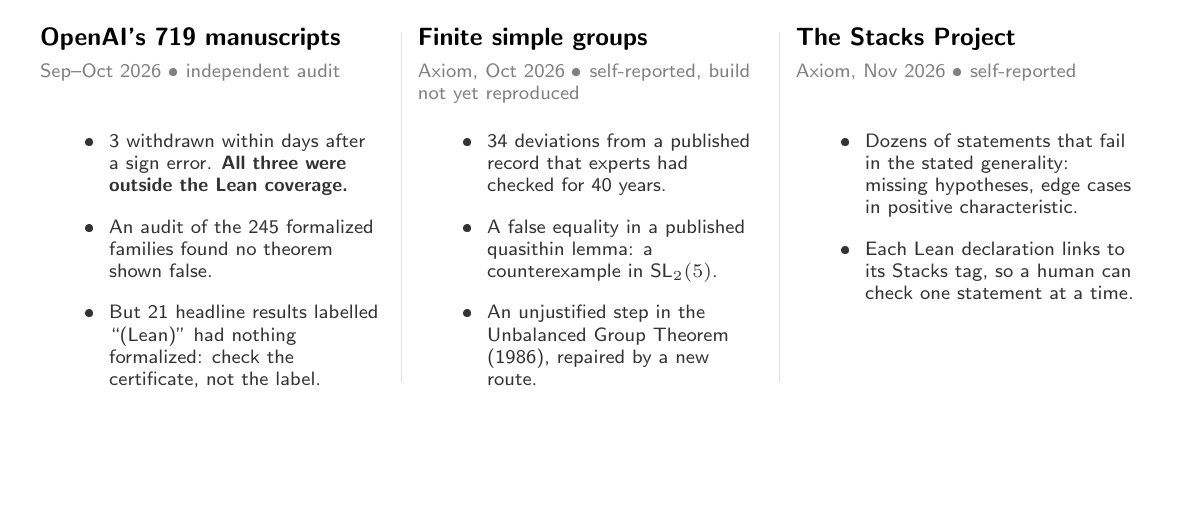
\begin{tikzpicture}[x=1cm, y=1cm,
      chead/.style={anchor=north west, text width=4.3cm, align=flush left, inner sep=0pt,
                    font=\sffamily\small\bfseries},
      ctag/.style={anchor=north west, text width=4.3cm, align=flush left, inner sep=0pt,
                   font=\sffamily\scriptsize, text=black!50},
      cbody/.style={anchor=north west, text width=4.3cm, align=flush left, inner sep=0pt,
                    font=\sffamily\scriptsize, text=black!80}]
    \useasboundingbox (0,0) rectangle (14.3,-5.9);
    \foreach \x in {4.75, 9.55} \draw[black!12, line width=0.5pt] (\x,-0.05) -- (\x,-4.5);
    % column 1
    \node[chead] at (0.15,0) {OpenAI's 719 manuscripts};
    \node[ctag] at (0.15,-0.45) {Sep--Oct 2026 \textbullet{} independent audit};
    \node[cbody] at (0.15,-0.95) {%
      \begin{itemize}\setlength{\itemsep}{3pt}
        \item 3 withdrawn within days after a sign error. \textbf{All three were outside the Lean coverage.}
        \item An audit of the 245 formalized families found no theorem shown false.
        \item But 21 headline results labelled ``(Lean)'' had nothing formalized: check the certificate, not the label.
      \end{itemize}};
    % column 2
    \node[chead] at (4.95,0) {Finite simple groups};
    \node[ctag] at (4.95,-0.45) {Axiom, Oct 2026 \textbullet{} self-reported, build not yet reproduced};
    \node[cbody] at (4.95,-0.95) {%
      \begin{itemize}\setlength{\itemsep}{3pt}
        \item 34 deviations from a published record that experts had checked for 40 years.
        \item A false equality in a published quasithin lemma: a counterexample in SL$_2(5)$.
        \item An unjustified step in the Unbalanced Group Theorem (1986), repaired by a new route.
      \end{itemize}};
    % column 3
    \node[chead] at (9.75,0) {The Stacks Project};
    \node[ctag] at (9.75,-0.45) {Axiom, Nov 2026 \textbullet{} self-reported};
    \node[cbody] at (9.75,-0.95) {%
      \begin{itemize}\setlength{\itemsep}{3pt}
        \item Dozens of statements that fail in the stated generality: missing hypotheses, edge cases in positive characteristic.
        \item Each Lean declaration links to its Stacks tag, so a human can check one statement at a time.
      \end{itemize}};
  \end{tikzpicture}
  \slidesources{borism/openai-math-slop, issue \#2 \textbullet{} OpenAI release record (Wikipedia) \textbullet{} Axiom, CFSG (Oct 2026) and Stacks (Nov 2026) \textbullet{} research note 01, \S\S2--3, 5}
\end{frame}

% [1 min] Navier--Stokes revisited, reframed in talk-v2 as auditability: the
% drift could be pinned to exact lemmas only because formal code existed.
% Originally: the certificate compiled, and the code
% still says something other than the paper. They do NOT claim the paper is
% wrong; the argument was about credit, not correctness.
\begin{frame}{The paper and the code disagree}
  \small\sffamily
  \begin{columns}[T]
    \begin{column}{0.54\textwidth}
      \textbf{Navier--Stokes} (Bastounis, Circelli \& Hansen, Oct 2026)
      \begin{itemize}\footnotesize
        \item The paper's estimate (8.19) needs $m{+}4$ derivatives; the matching Lean theorem assumes $m{+}5$, and the pattern repeats.
        \item The paper's pressure bound depends on one quantity; the Lean bound depends on two, and is proved by a different route.
        \item They do not claim the paper is wrong.
      \end{itemize}
      \medskip
      \textbf{OpenAI's 719 manuscripts} (community audit of 245 formalized families)
      \begin{itemize}\footnotesize
        \item About 210 consistent at the level of statements; no theorem shown false.
        \item 21 headline results marked ``(Lean)'' were not formalized; 5 formalized only a supporting lemma.
      \end{itemize}
    \end{column}
    \begin{column}{0.42\textwidth}
      \vspace{0.4cm}
      \begin{tikzpicture}
        \node[draw=PennRed!45, fill=PennRed!3, line width=0.6pt, rounded corners=2pt,
              text width=5.3cm, inner sep=0.3cm, align=left, font=\rmfamily\itshape\small] (q)
          {Lean acceptance (compilation) of translation does not imply semantic preservation.};
        \node[anchor=north west, font=\sffamily\scriptsize, text=black!60, inner sep=0pt]
          at ([yshift=-0.15cm]q.south west) {--- Bastounis, Circelli \& Hansen, arXiv 2610.08144};
      \end{tikzpicture}
      \vspace{0.5cm}

      {\footnotesize The drift was found because there was formal code to hold the paper against.\par\smallskip
       A certificate proves \emph{a} theorem. Whether it is \emph{the} theorem is a human question.}
    \end{column}
  \end{columns}
  \slidesources{Bastounis, Circelli \& Hansen, arXiv 2610.08144 \textbullet{} borism/openai-math-slop, issue \#2 \textbullet{} research note 01, \S5}
\end{frame}

% [2 min] Who did what, and who is told. Each row: the problem, the case that
% exposed it, the institutional response, and how far that response reaches.
\begin{frame}{Credit, disclosure and confidentiality}
  \footnotesize\sffamily
  \renewcommand{\arraystretch}{1.35}
  \begin{tabularx}{\linewidth}{@{}p{2.3cm}YYp{1.5cm}@{}}
    \toprule
    \tabhead{Problem} & \tabhead{Case} & \tabhead{Response} & \tabhead{Status}\\
    \midrule
    \rowhead{Credit} & AI reuses known ideas without attribution: 8 of Aletheia's 13 meaningful Erd\H{o}s results were already in the literature. Kolda: ``Human--AI scrapple''
      & Leiden Declaration (Jun 2026, endorsed by the IMU): human responsibility, attribution & \stpartial\\
    \rowhead{Priority} & Navier--Stokes priority dispute (C\'ordoba \& Mart\'inez-Zoroa; Buckmaster \& Alp\"oge)
      & AGMAI release guidelines (29 Sep): review before announcement, release prompts. Labs withheld prompts & \stopen\\
    \rowhead{Disclosure} & 1 in 6 math preprints read as AI-written without saying so. At ICML 2026, 22.5\% of reviewers used an LLM under a ban
      & Disclosure statements (arXiv, Springer, Leiden); SIAM AI policy v2.0 & \stpartial\\
    \rowhead{Confidentiality} & Referees uploading manuscripts to AI tools
      & LMS: misconduct. SIAM v2.0: ``non-delegation of scholarly judgement'' & \stpartial\\
    \bottomrule
  \end{tabularx}\par\medskip
  {\color{black!60}\scriptsize The rules already bind individuals; none of them can be checked from the paper alone.}
  \slidesources{Reisinger et al., AcadMathSci, Oct 2026 (A.3, C.1, C.4, C.5) \textbullet{} Kolda, Silicon Reckoner, Feb 2026 \textbullet{} K.~Martin, \emph{AI use in arXiv mathematics papers} (3 Nov 2026) \textbullet{} Kim et al., arXiv 2609.19420}
\end{frame}

% [1.5 min] Who learns, who can afford it, and what gets studied.
\begin{frame}{Training, access and narrowing}
  \footnotesize\sffamily
  \renewcommand{\arraystretch}{1.35}
  \begin{tabularx}{\linewidth}{@{}p{2.3cm}YYp{1.5cm}@{}}
    \toprule
    \tabhead{Problem} & \tabhead{Case} & \tabhead{Response} & \tabhead{Status}\\
    \midrule
    \rowhead{Training} & Students given unrestricted GPT-4 scored 17\% lower once access was removed; a tutor with guardrails largely avoided the harm (Bastani et al.)
      & Vivas and in-person exams; AI-permitted work graded on formulation and validation & \stpartial\\
    \rowhead{Access} & Only 11\% of researchers have institutional funding for their main AI tool (Springer Nature, 10,480 researchers). Navier--Stokes cost an estimated \pounds4.9M
      & Token costs eligible on grants (proposed); SAIR Open Math OS: free open models for academics & \stpartial\\
    \rowhead{Narrowing} & AI adoption shrinks topic range by 4.6\% and engagement by 22\% (Hao et al., 41M papers). Agendas drift toward ``problems easily amenable to current AI''
      & Reward understanding and long-term contribution over volume (AcadMathSci) & \stopen\\
    \bottomrule
  \end{tabularx}
  \slidesources{Reisinger et al., AcadMathSci, Oct 2026 (\S1.6, \S3.2, \S3.3, \S4.3, B.1) \textbullet{} Bastani et al., PNAS \textbullet{} Hao et al., arXiv 2412.07727}
\end{frame}

\begin{frame}{Corpus and scoring method}
  \stub{--}{Details behind the opinion map}
\end{frame}

\begin{frame}{Backup slides}
  \stub{--}{Material for questions}
\end{frame}

\begin{frame}{References}
  \stub{--}{Sources}
\end{frame}
